Organize this section according to the rules defined in the project description. 

\subsection{External Interface Requirements}
\subsubsection{User interfaces}
\subsubsection{Hardware Interfaces}
\subsubsection{Software Interfaces}
\subsubsection{Communication Interfaces}
\subsection{Functional requirements}
% Definition  of  use  case  diagrams,  use  cases  and  associated sequence/activity diagrams, and mapping on requirements 

\begin{figure}
	\centering
	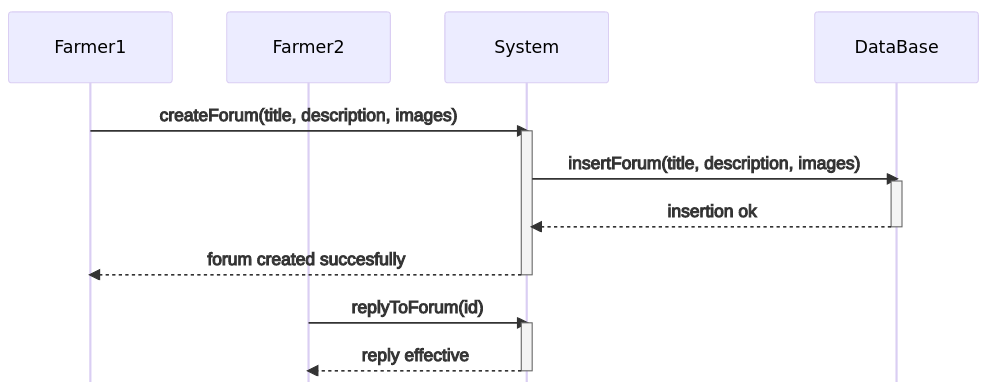
\includegraphics[width=\textwidth]{Images/seq-create-forum.png}
	\caption{\label{fig:seqcreationforum} Sequence diagram on the creation of a forum and the reply by another farmer}
\end{figure}

\begin{figure}
	\centering
	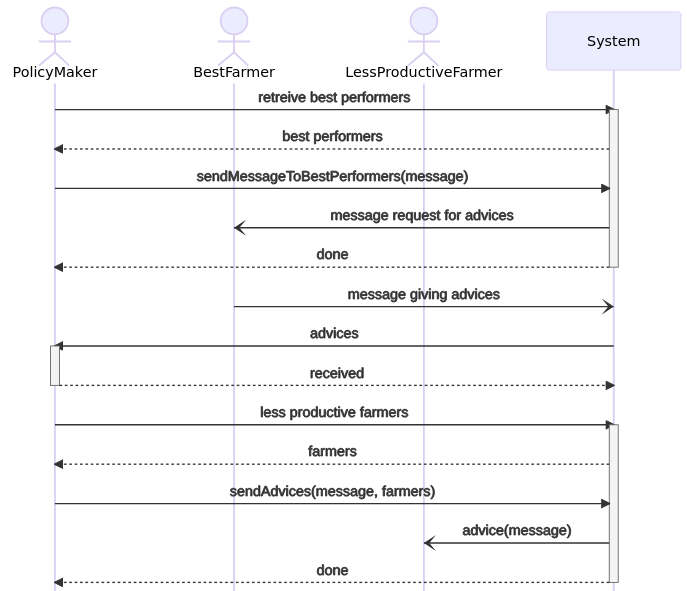
\includegraphics[width=\textwidth]{Images/seq-policy-farmers.png}
	\caption{\label{fig:seq} Sequence diagram showing a policy marker reaching out best performing farmers for advises and send them to less productive farmer}
\end{figure}

\subsection{Performance Requirements}

\subsection{Design Constraints}
\subsubsection{Standards compliance}
\subsubsection{Hardware limitations}
\subsubsection{Any other constraint ??}
Do we keep it ?
\subsection{Software System Attributes}
\subsubsection{Reliability}
\subsubsection{Availability}
\subsubsection{Security}
\subsubsection{Maintainability}
\subsubsection{Portability}
